\documentclass[]{article}
\usepackage{lmodern}
\usepackage{amssymb,amsmath}
\usepackage{ifxetex,ifluatex}
\usepackage{fixltx2e} % provides \textsubscript
\ifnum 0\ifxetex 1\fi\ifluatex 1\fi=0 % if pdftex
  \usepackage[T1]{fontenc}
  \usepackage[utf8]{inputenc}
\else % if luatex or xelatex
  \ifxetex
    \usepackage{mathspec}
  \else
    \usepackage{fontspec}
  \fi
  \defaultfontfeatures{Ligatures=TeX,Scale=MatchLowercase}
\fi
% use upquote if available, for straight quotes in verbatim environments
\IfFileExists{upquote.sty}{\usepackage{upquote}}{}
% use microtype if available
\IfFileExists{microtype.sty}{%
\usepackage[]{microtype}
\UseMicrotypeSet[protrusion]{basicmath} % disable protrusion for tt fonts
}{}
\PassOptionsToPackage{hyphens}{url} % url is loaded by hyperref
\usepackage[unicode=true]{hyperref}
\hypersetup{
            pdftitle={Guías para Implementación de Filtro Sanitario},
            pdfborder={0 0 0},
            breaklinks=true}
\urlstyle{same}  % don't use monospace font for urls
\usepackage[margin=1in]{geometry}
\usepackage{graphicx,grffile}
\makeatletter
\def\maxwidth{\ifdim\Gin@nat@width>\linewidth\linewidth\else\Gin@nat@width\fi}
\def\maxheight{\ifdim\Gin@nat@height>\textheight\textheight\else\Gin@nat@height\fi}
\makeatother
% Scale images if necessary, so that they will not overflow the page
% margins by default, and it is still possible to overwrite the defaults
% using explicit options in \includegraphics[width, height, ...]{}
\setkeys{Gin}{width=\maxwidth,height=\maxheight,keepaspectratio}
\IfFileExists{parskip.sty}{%
\usepackage{parskip}
}{% else
\setlength{\parindent}{0pt}
\setlength{\parskip}{6pt plus 2pt minus 1pt}
}
\setlength{\emergencystretch}{3em}  % prevent overfull lines
\providecommand{\tightlist}{%
  \setlength{\itemsep}{0pt}\setlength{\parskip}{0pt}}
\setcounter{secnumdepth}{0}
% Redefines (sub)paragraphs to behave more like sections
\ifx\paragraph\undefined\else
\let\oldparagraph\paragraph
\renewcommand{\paragraph}[1]{\oldparagraph{#1}\mbox{}}
\fi
\ifx\subparagraph\undefined\else
\let\oldsubparagraph\subparagraph
\renewcommand{\subparagraph}[1]{\oldsubparagraph{#1}\mbox{}}
\fi

% set default figure placement to htbp
\makeatletter
\def\fps@figure{htbp}
\makeatother

\usepackage{etoolbox}
\makeatletter
\providecommand{\subtitle}[1]{% add subtitle to \maketitle
  \apptocmd{\@title}{\par {\large #1 \par}}{}{}
}
\makeatother

\title{Guías para Implementación de Filtro Sanitario}
\providecommand{\subtitle}[1]{}
\subtitle{Asociación de Baja California, Iglesia Adventista del Séptimo Día}
\author{}
\date{\vspace{-2.5em}24 de Mayo de 2020}

\begin{document}
\maketitle

Éste documento ha sido compilado utilizando como guía el
documentoproporcionado por el Dr.~Donatt en la sesión del miércoles 20
de Mayo del 2020, se ha complementado con implementaciones
personalizadas para la Asociación de Baja California de los Adventistas
del Séptimo Día.

\textbf{El filtro sanitario se debe implementar en las fases de semáforo
amarillas y verdes en todos los centros de culto.}

\subsection{Logística de
Actividades:}\label{loguxedstica-de-actividades}

\begin{enumerate}
\def\labelenumi{\arabic{enumi}.}
\tightlist
\item
  A la entrada o entradas de cada recinto cerrado deberá delimitarse una
  zona de recepción con marcas definidas en el piso o barreras.

  \begin{itemize}
  \tightlist
  \item
    Este Filtro deberá ser atendido por el personal previamente
    capacitado que se designe.
  \item
    Toda persona que desee entrar al recinto deberá portar correctamente
    un cubre boca propio, si no lo está portando de manera correcta, se
    le orientará para que lo corrija.
  \end{itemize}
\item
  Tomar la temperatura corporal:

  \begin{itemize}
  \tightlist
  \item
    Deberá ser tomada a distancia a cada persona con un termómetro
    digital infrarrojo bien calibrado.
  \item
    Si la persona tiene una temperatura mayor o igual a 38 grados
    Centígrados, no continuará con los siguientes pasos y no podrá
    permanecer en el lugar. Recomendándole acudir a una evaluación
    médica.
  \item
    Si la persona presenta una temperatura corporal menor a 38 grados
    Centígrados, podrá avanzar al siguiente paso.
  \item
    La temperatura aceptable se deberá anotar en el cuestionario que se
    entregará a cada persona.
  \end{itemize}
\item
  Dentro de la zona marcada como filtro, debe existir:

  \begin{itemize}
  \tightlist
  \item
    Una charola, bandeja o tapete impregnados o que contengan una
    solución de Hipoclorito de Sodio para que, al pisarlo, desinfecte la
    suela de los zapatos.
  \item
    Una toalla de piso seca o tapete absorbente para pisar después del
    Hipoclorito y secar los excedentes.
  \item
    En su defecto, se le proporcionara a cada persona un par de cubre
    zapatos para poder continuar.
  \item
    Proporcionar o aplicar a cada persona, gel desinfectante de alcohol
    al 70\% para desinfectar sus manos antes de tocar cualquier otra
    cosa y a la salida del recinto.
  \end{itemize}
\item
  Entregar un boligrafo y una hoja que contenga un cuestionario que
  indique su estado de salud actual.

  \begin{itemize}
  \tightlist
  \item
    A continuación se presenta el formato del cuestionario impreso a
    utilizarse:
  \end{itemize}
\end{enumerate}

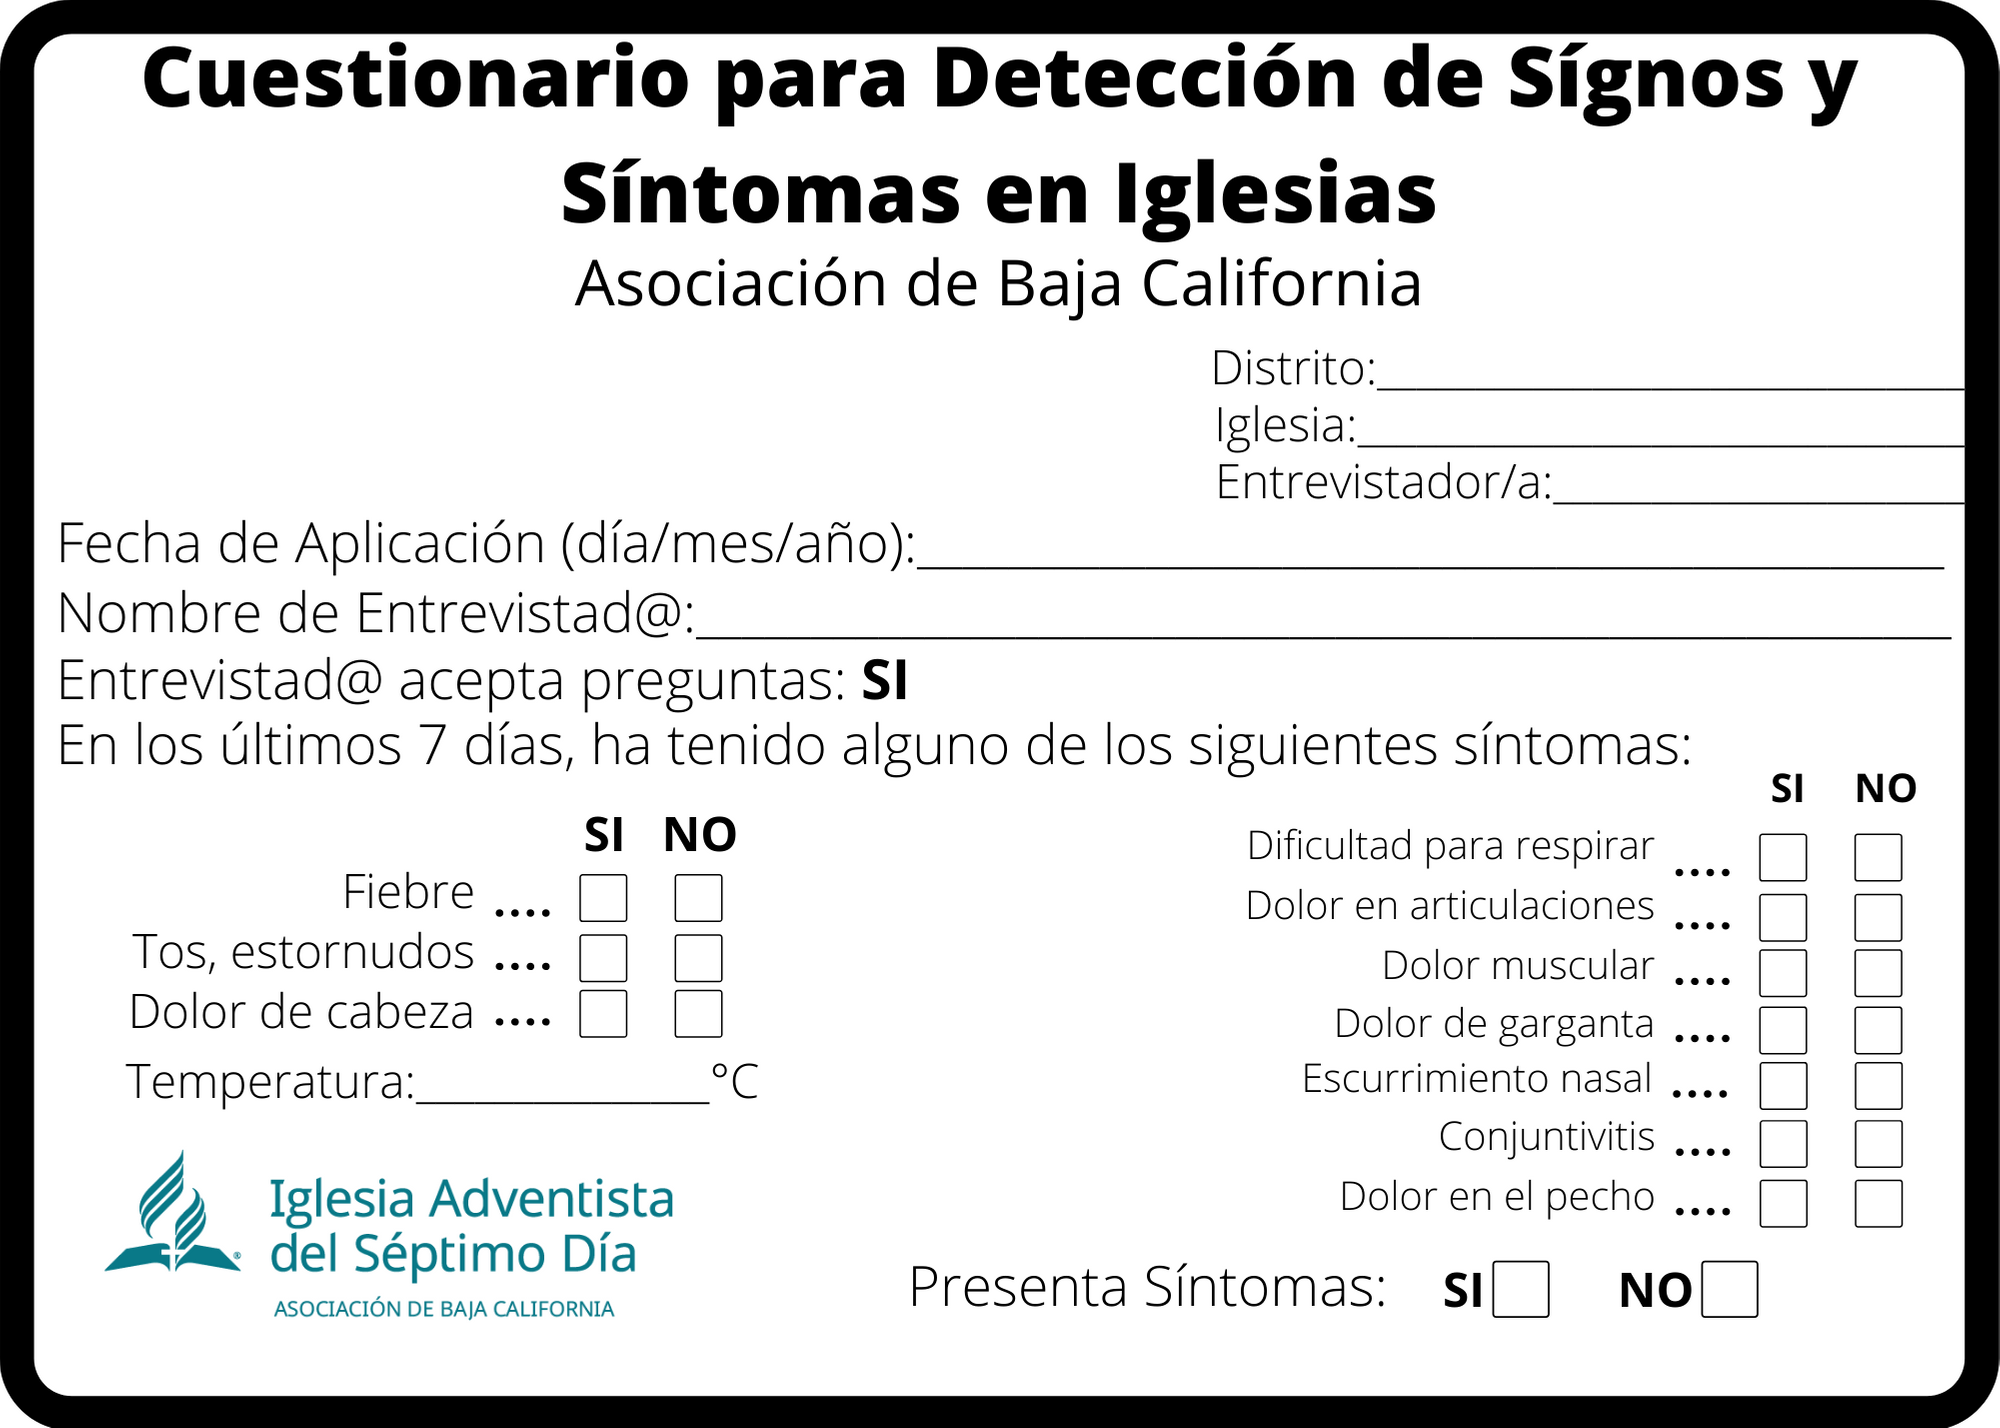
\includegraphics[width=5.20833in]{data/img/1.png}

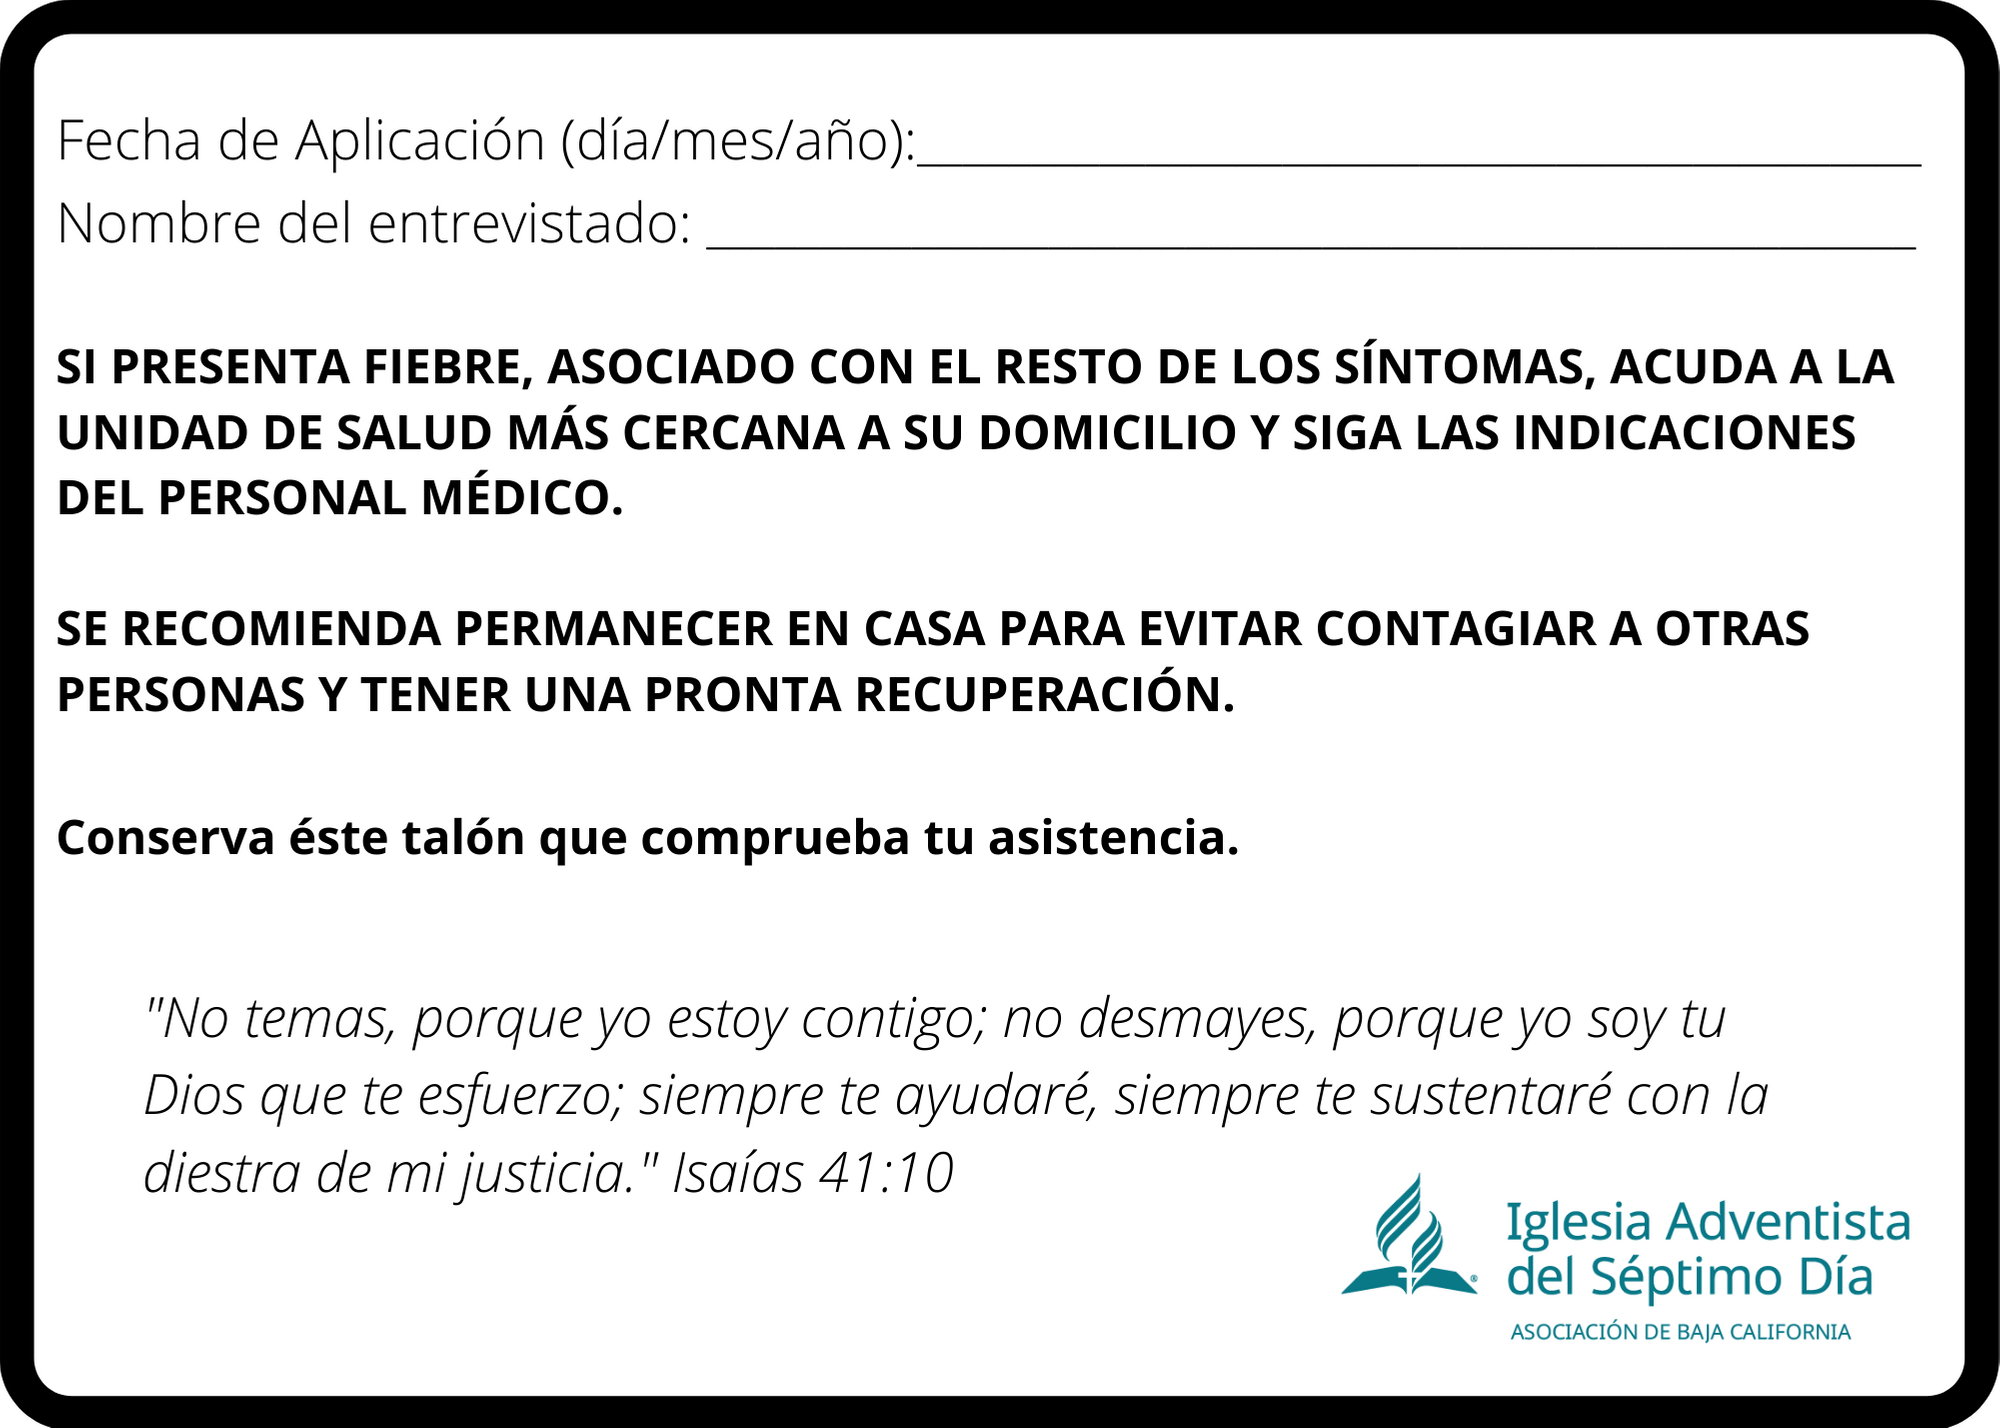
\includegraphics[width=5.20833in]{data/img/2.png}

\subsection{Requerimientos Necesarios}\label{requerimientos-necesarios}

\begin{enumerate}
\def\labelenumi{\arabic{enumi}.}
\tightlist
\item
  Designar y adiestrar a miembros voluntarios de la Iglesia para atender
  el filtro sanitario.

  \begin{itemize}
  \tightlist
  \item
    Pueden participar: profesionales de la salud o personas capacitadas.
  \item
    La capasitación deberá ser proporcionada por profesionales de la
    salud.
  \item
    Podrán ser capacitados, los Guias Mayores, las Diaconizas, los
    Diaconos o toda persona que se ofresca como voluntaria y que
    acredite la capacitación.
  \end{itemize}
\item
  Cada persona que atienda el Filtro Sanitario, deberá vestir el
  siguiente equipo:

  \begin{itemize}
  \tightlist
  \item
    Bata protectora de tela o desechable.
  \item
    Cubre boca
    \href{https://www.bypmedical.com.mx/producto/cubrebocas-tricapa-fda/}{tricapa}.
  \item
    Lentes de protección y/o Careta de acetato que cubra toda su cara.
  \item
    Guantes de
    \href{https://www.homedepot.com.mx/seguridad/equipo-de-seguridad/guantes/guante-de-latex-desechable-10-piezas-133909}{Latex}
    o
    \href{https://www.homedepot.com.mx/seguridad/equipo-de-seguridad/guantes/guante-nitrilo-desechable-107411}{Nitrilo}
    o
    \href{http://rygsac.com/indumentaria-de-un-solo-uso/alimentario-de-un-solo-uso/guantes-de-polietileno}{Polietileno}
    no esteriles.
  \end{itemize}
\item
  La Iglesia deberá proporcionar los Equipos de Protección Personal
  (EPP), mencionados en el punto anterior, al personal capacitado que
  atenderá el filtro sanitario.

  \begin{itemize}
  \tightlist
  \item
    El EPP deberá ser lavable o desechable con excepción de los Googles
    de protección y/o Caretas de acetato.
  \end{itemize}
\item
  Deberá tener una mesa o escritorio cubierto con un paño de tela
  lavable o plastico desechable. En caso de no disponer de esto, se
  deberá limpiar la superficie cada 4 horas con una solución diluida de
  Hipoclorito de Sodio:
\end{enumerate}

\includegraphics[width=2.60417in]{https://pbs.twimg.com/media/D2WpmFDX4AAEjyy.jpg}

\begin{enumerate}
\def\labelenumi{\arabic{enumi}.}
\tightlist
\item
  Deberá tener sillas para los encargados de aplicar el Filtro Sanitario
  y estas se ubicarán con un metro y medio de separación entre silla y
  silla.
\item
  Deberá tener una charola, bandeja o tapete impregnados o que contengan
  una solución de Hipoclorito de Sodio para que, al pisarlo, desinfecte
  la suela de los zapatos.

  \begin{itemize}
  \tightlist
  \item
    Una toalla de piso seca o tapete absorbente para pisar después del
    Hipoclorito y secar los excedentes.
  \item
    En su defecto, se le proporcionara a cada persona un par de cubre
    zapatos para poder continuar.
  \end{itemize}
\item
  Deberá haber agua y jabón o bien gel desinfectante de alcohol al 70\%
  y una solución clorada (Hipoclorito se Sodio) para mantener limpio y
  desinfectado.
\item
  Deberá tener toallas de papel desechables.
\item
  Deberá tener un bote para basura con bolsa plástica desechable y con
  tapa, para los desechos (se deberá evitar la acumulación de los
  desechos).
\item
  Deberá tener un termómetro digital infrarrojo.
\item
  Deberá tener suficientes cuestionarios de detección y bolígrafos.
\item
  Antes de vestir el EPP se deberá desinfectar las manos con gel de
  alcohol al 70\% o con agua y jabón.

  \begin{itemize}
  \tightlist
  \item
    Se deberá colocar de manera correcta el cubre bocas, cubriendo boca
    y nariz, asegurando que no haya espacios entre su cara y el cubre
    bocas.
  \item
    Debe evitar tocarse el cubre boca mientras lo usa; si lo hace,
    deberá lavarse las manos nuevamente.
  \item
    Deberá cambiar el cubre boca tan pronto como esté húmedo y no
    reutilizarlo si es desechable.
  \item
    Para quitar el cubre boca deberá tomarlo por atrás (nunca por la
    parte delantera) y depositarlo en un recipiente cerrado, y lavar las
    manos nuevamente.
  \item
    Si el cubre boca es lavable, deberá lavarlo con agua y jabón después
    de usarlo y volver a usarlo hasta que esté completamente seco.
  \item
    Recuerda que el uso de cubre bocas no sustituye a las otras medidas
    de protección.
  \end{itemize}
\item
  Después de la colocación del cubre bocas, deberá vestir los demás
  implementos de protección.

  \begin{itemize}
  \tightlist
  \item
    Deberá vestir la bata u overol con gorro.
  \item
    Colocarse los googles de protección y/o la careta de acetato
  \item
    Al final los guantes de látex, o nitrilo, o polietileno.
  \end{itemize}
\end{enumerate}

\subsection{Recabado de información e
Informes}\label{recabado-de-informaciuxf3n-e-informes}

Se propone recabar el filtro sanitario en el siguiente repositorio en
línea:

\begin{itemize}
\tightlist
\item
  \url{https://forms.gle/CitYXr1ts8tcvniM8}
\end{itemize}

Ésto permitirá el análisis en tiempo y forma para la toma de decisiones
por parte de los directivos en la Asociación de Baja California que así
mejor convengan para afrontar la crisis que representa ésta pandemia.

En colaboración con la adminsitración de la Asociación de Baja
California se ha generado también la georeferenciación de las iglesias
en los 3 campos de la misma, ésto con el objetivo de presentar análisis
apropiados para la toma de decisiones en tiempo cuasi-real. Ofreciendo a
los dirigentes una ventaja competitiva \emph{versus} el uso únicamente
de filtros sanitarios en físico.

En los siguientes mapas se muestran las iglesias por distrito y/o área.
Se pueden generar visualizaciones por cada distrito o por regiones en
particular con los nombres de cada iglesia, se ha evitado hacer ésto de
inicio para proteger la privacidad de los datos de las iglesias. Previa
solicitud del equipo administrativo de la Asociación de Baja California
los datos se pueden desplegar para la toma de decisiones.

\subsubsection{Iglesias Tijuana}\label{iglesias-tijuana}

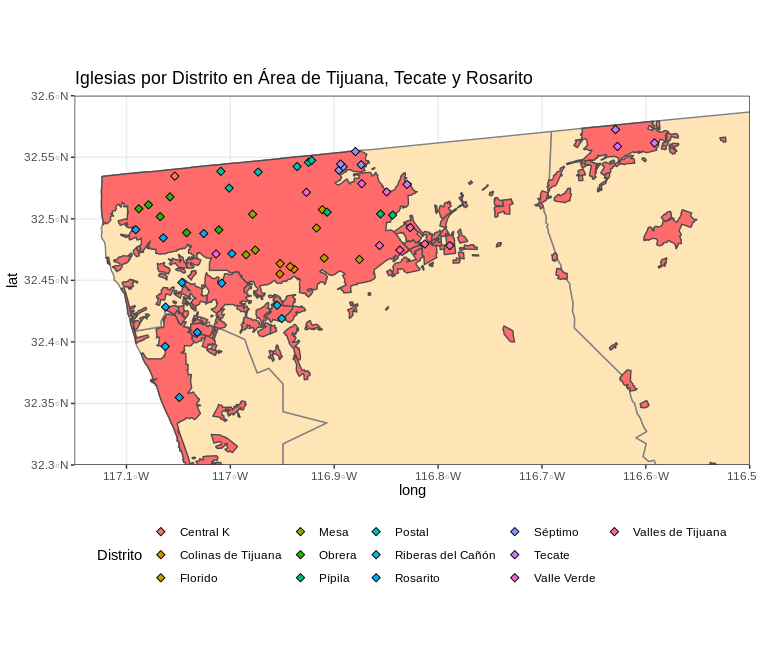
\includegraphics[width=5.20833in]{img/iglesiasTijuana.png}

No fué posible geolocalizar (encontrar sus coordenadas en google maps)
las siguientes iglesias:

\begin{enumerate}
\def\labelenumi{\arabic{enumi}.}
\tightlist
\item
  Colinas de Tijuana:

  \begin{itemize}
  \tightlist
  \item
    Centenario.
  \item
    Cuauhtemoc.
  \item
    Los Pinos.
  \end{itemize}
\item
  Florido:

  \begin{itemize}
  \tightlist
  \item
    Los Olivos.
  \end{itemize}
\item
  Mesa:

  \begin{itemize}
  \tightlist
  \item
    Internacional.
  \end{itemize}
\item
  Pípila:

  \begin{itemize}
  \tightlist
  \item
    El Pípila.
  \item
    El Barretal.
  \end{itemize}
\item
  Séptimo:

  \begin{itemize}
  \tightlist
  \item
    Rinconada II.
  \item
    La Frontera.
  \end{itemize}
\item
  Valle Verde:

  \begin{itemize}
  \tightlist
  \item
    Chilpancingo.
  \end{itemize}
\item
  Valles de Tijuana:

  \begin{itemize}
  \tightlist
  \item
    Vistas del Valle.
  \item
    Los Laureles.
  \item
    Los Girasoles.
  \end{itemize}
\item
  Central K:

  \begin{itemize}
  \tightlist
  \item
    Cárdenas.
  \end{itemize}
\item
  Postal:

  \begin{itemize}
  \tightlist
  \item
    Tzotzil.
  \end{itemize}
\item
  Riberas del Cañón:

  \begin{itemize}
  \tightlist
  \item
    La Presa/Los Pinos.
  \end{itemize}
\item
  Rosarito:

  \begin{itemize}
  \tightlist
  \item
    Las Cruces.
  \item
    Xico.
  \end{itemize}
\item
  Tecate:

  \begin{itemize}
  \tightlist
  \item
    Hongo.
  \item
    San Pedro.
  \end{itemize}
\end{enumerate}

Será importante tener el apoyo de los pastores locales o la
administración central para geolocalizar las iglesias anteriores.

\subsection{Iglesias Mexicali y San Luis Río
Colorado}\label{iglesias-mexicali-y-san-luis-ruxedo-colorado}

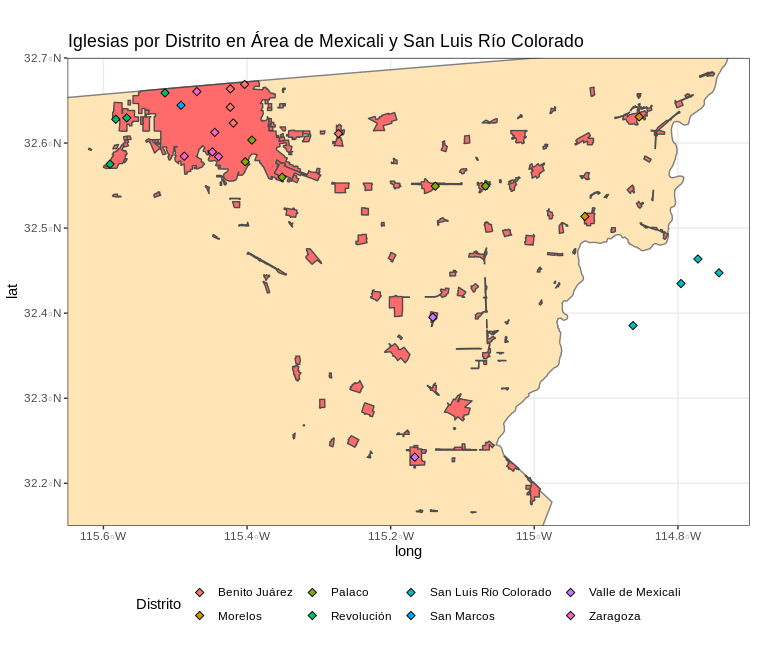
\includegraphics[width=5.20833in]{img/iglesiasMexicali.png}

No fué posible geolocalizar (encontrar sus coordenadas en google maps)
las siguientes iglesias:

\begin{enumerate}
\def\labelenumi{\arabic{enumi}.}
\tightlist
\item
  Palaco:

  \begin{itemize}
  \tightlist
  \item
    Monarcas.
  \item
    Venustiano Carranza.
  \end{itemize}
\item
  Revolución:

  \begin{itemize}
  \tightlist
  \item
    Colosio.
  \end{itemize}
\item
  San Marcos:

  \begin{itemize}
  \tightlist
  \item
    Pueblo Nuevo.
  \item
    Fundadores.
  \end{itemize}
\item
  Morelos:

  \begin{itemize}
  \tightlist
  \item
    5 de Mayo.
  \item
    Ejido Benito Juárez.
  \item
    Ladrillera.
  \item
    Lázaro Cárdenas.
  \end{itemize}
\item
  Valle de Mexicali:

  \begin{itemize}
  \tightlist
  \item
    Ejido Durango.
  \item
    Ejido Veracruz.
  \item
    Ejido Km 57.
  \end{itemize}
\end{enumerate}

\subsection{Iglesias Ensenada}\label{iglesias-ensenada}

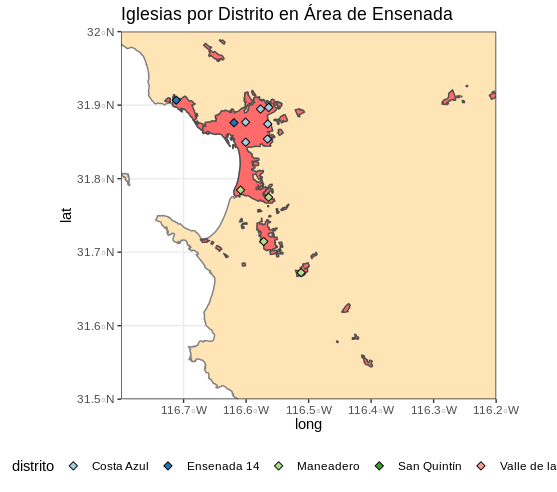
\includegraphics[width=5.20833in]{img/iglesiasEnsenada.png}

No fué posible geolocalizar (encontrar sus coordenadas en google maps)
las siguientes iglesias:

\begin{enumerate}
\def\labelenumi{\arabic{enumi}.}
\tightlist
\item
  Ensenada 14:

  \begin{itemize}
  \tightlist
  \item
    Loma Linda.
  \item
    Flores Magón.
  \end{itemize}
\item
  Maneadero:

  \begin{itemize}
  \tightlist
  \item
    San Vicente.
  \end{itemize}
\end{enumerate}

\subsection{Iglesias San Quintín y Valle de la
Trinidad}\label{iglesias-san-quintuxedn-y-valle-de-la-trinidad}

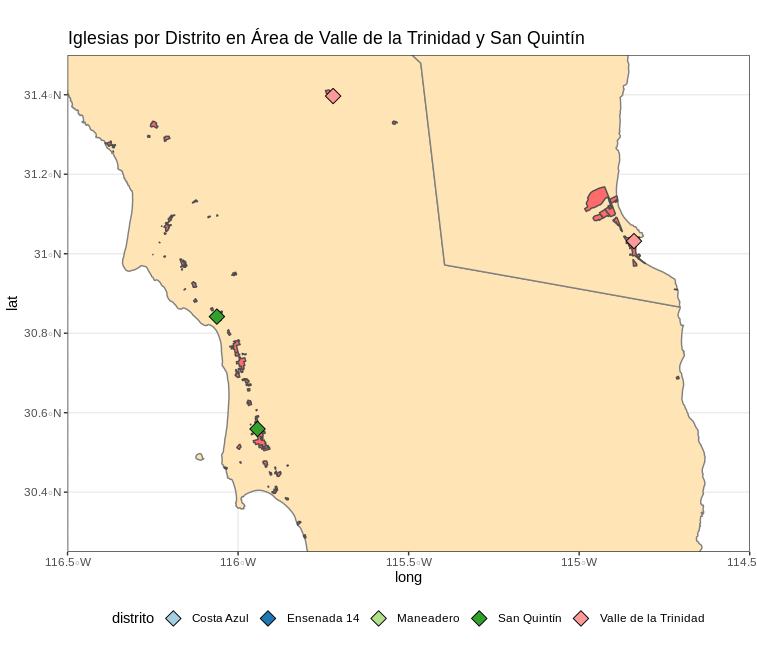
\includegraphics[width=5.20833in]{img/iglesiasSQVT.png}

No fué posible geolocalizar (encontrar sus coordenadas en google maps)
las siguientes iglesias:

\begin{enumerate}
\def\labelenumi{\arabic{enumi}.}
\tightlist
\item
  San Quintín:

  \begin{itemize}
  \tightlist
  \item
    Zapata.
  \item
    Leandro Valle.
  \item
    El Rosario.
  \item
    Colonet.
  \end{itemize}
\item
  Valle de la Trinidad:

  \begin{itemize}
  \tightlist
  \item
    Héroes de la Independencia.
  \item
    El Oasis.
  \item
    San Matías.
  \end{itemize}
\end{enumerate}

\end{document}
